\documentclass[10pt,oneside]{article}

% Fonts and language
\usepackage[utf8]{inputenc}
\usepackage[vietnamese,english]{babel} % Hỗ trợ tiếng Việt
\usepackage[T5]{fontenc}
\usepackage{mathptmx} % Sử dụng Times New Roman
\usepackage[hidelinks]{hyperref}
\usepackage{longtable}
\usepackage{geometry}
\geometry{
    a4paper,
    left=1.2cm,
    right=2.1cm,
    top=1.6cm,
    bottom=1.1cm
}
\usepackage{fancyhdr}

\usepackage[en-GB]{datetime2}

% to have awesome icon 
\usepackage{fontawesome} 
\usepackage{academicons}

\usepackage{tcolorbox}
\usepackage{tikz}
\usepackage{array}
\newcolumntype{P}[1]{>{\centering\arraybackslash}p{#1}}
\usepackage{lipsum}

\usepackage{caption}
\captionsetup{justification=raggedright,singlelinecheck=false,font={Large, bf}}
% pictures
\usepackage{graphicx}
\graphicspath{{./Figs/}}

% Picture & current 

\newcommand{\itemlike}[2]
{
    \begin{tabular*}{1\textwidth}{p{2.5cm} p{8cm}}
    ~\normalsize{{ \color{orange} #1:}} & #2\\ [3pt]
    \end{tabular*}
}

\newcommand{\experience}[4]
{
    \textbf{#1} \hfill  \faMapMarker \textit{ #3} \newline
    \textit{#2} \newline
    #4 \\ \\ 
}

\newcommand{\publication}[4]
{
    \textbf{#1}\newline #2 & \textbf{#3} #4\\ \\
}

\DTMsavedate{born}{2002-05-24}

\newcommand{\authorname}{Đặng Thị Mỹ Ly }

\begin{document}

\pagestyle{fancy}
\thispagestyle{empty}
\fancyhead[L]{\authorname - Curriculum Vitae}
\fancyhead[R]{\today}

\begin{center}
{\LARGE{\textbf{\authorname}} - Curriculum Vitae} \\
\small{\today}
\end{center}


\begin{tcolorbox}[
    sidebyside,
    righthand width = 0.2\columnwidth,
    colback = white, 
    colframe = white,
    coltitle=black,
]
\itemlike{Ngày sinh}{\DTMusedate{born}}
\itemlike{Trạng thái}{Sinh viên năm 4, Trường đại học Sài Gòn}
\itemlike{Lĩnh vực}{Kỹ thuật phần mềm}
\itemlike{Công cụ}{ApacheNetBeans,Eclipse,AndroidStudio - Java \newline SQL Server - SQL}
%\itemlike{Activities}{Activity 1, Activity 2} % optional
\itemlike{Liên hệ}{TP.Hồ Chí Minh  \newline 0981613951 \newline \href{mailto:your.email@your.domain}{myylyy12@gmail.com} }
\tcblower
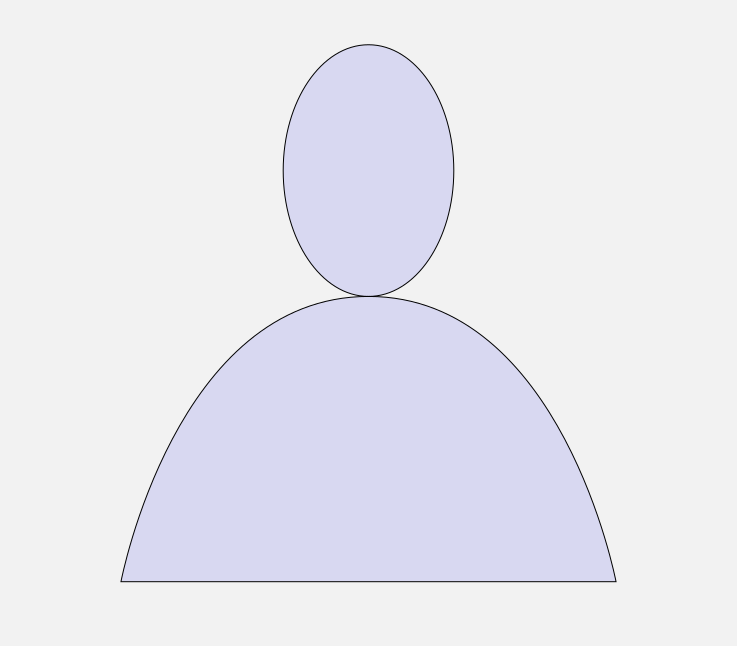
\includegraphics[width=\columnwidth]{Figs/CVdummy.png} 
\end{tcolorbox}


%\vspace{0.5cm} 

\vspace{0.5cm}

\begin{longtable}{p{0.2\columnwidth} p{0.8\columnwidth}}
    \caption*{Work experience}\\
    \hline\\
    2024 & \experience{}{}{
    Chưa có kinh nghiệm làm việc
    }
  
\end{longtable}

\begin{longtable}{p{0.2\columnwidth} p{0.8\columnwidth}}
    \caption*{Education}\\
    \hline\\
    2020-present & \experience{Bằng Cử nhân}{Trường đại học Sài Gòn}{TP.Hồ Chí Minh, Việt Nam}{
    
    }
\end{longtable}



\begin{longtable}{p{0.2\columnwidth} p{0.8\columnwidth}}
    \caption*{Kỹ năng Công Nghệ Thông Tin}\\
    \hline\\
    \textbf{Softwares} & Apache NetBeans: Advanced \newline SQL Server: Intermediate \newline Visual Studio Code: Advanced \newline
    Android Studio: Intermediate \\ \\
    
    \textbf{Programming} & Python: beginner \newline Java: Advanced \newline C/C++:  beginner \newline SQL: Intermediate \newline JavaScripts : beginner \\ \\
    
    \textbf{Office} & Microsoft office tools: Intermediate \newline \LaTeX: beginner \\
    
\end{longtable}

\end{document}
